\chapter{Literature Survey}

\section{Foundations of Grammatical Error Correction}

\subsection{Definition and Scope of GEC}

Grammatical Error Correction (GEC) is a Natural Language Processing (NLP) task concerned with automatically transforming erroneous sentences into grammatically acceptable forms while preserving intended meaning \cite{ng-etal-2014-conll}. Earlier work often focused on morpho-syntactic violations such as subject--verb agreement, tense errors, article misuse, and word order \cite{bryant-etal-2017-automatic}. More recent systems address a wider range of issues, including spelling, punctuation, lexical choice, and limited sentence restructuring \cite{10.1162/coli_a_00478}. In practice, this means that GEC sits close to writing improvement, even though the two tasks are not the same.

The literature commonly distinguishes between \textit{grammaticality}, \textit{fluency}, and \textit{style} \cite{napoles-etal-2017-jfleg}. Grammaticality concerns conformity to linguistic rules, fluency refers to naturalness and readability, and style reflects authorial preference rather than correctness. Modern neural systems increasingly optimise for fluency, often producing broader rewrites rather than minimal edits \cite{loem2023exploringeffectivenessgpt3grammatical}. This creates a practical difficulty for GEC: a sentence may sound better after correction while also moving away from the learner's own wording. The distinction between grammatical correction and writing enhancement therefore matters for both evaluation and learner feedback \cite{ke2019automated}.

\subsection{Historical Evolution of GEC Systems}

GEC has developed alongside wider changes in NLP, moving from rule-based systems to statistical models and, more recently, large-scale neural architectures \cite{10.1162/coli_a_00478}.

\subsubsection{Rule-Based Systems}

Early GEC systems relied on hand-crafted linguistic rules designed to detect and correct specific error types. These systems typically targeted well-defined morpho-syntactic phenomena, such as subject--verb agreement, article usage, and verb tense errors \cite{ng-etal-2014-conll}. Rule-based approaches offered interpretability and precise control over corrections, but they were limited by coverage. Building and maintaining large rule sets required linguistic expertise, and such systems struggled when learner errors fell outside predefined categories \cite{10.1162/coli_a_00478}.

\subsubsection{Statistical Machine Translation (SMT)-Based GEC}

Statistical Machine Translation (SMT) changed the way GEC was framed. Rather than treating correction as isolated rule application, SMT-based approaches treated it as a monolingual translation task, converting ``incorrect'' sentences into corrected counterparts \cite{brockett2006correcting}. This allowed systems to learn correction patterns from parallel corpora of learner text and annotated revisions.

SMT approaches improved flexibility and coverage compared to rule-based systems \cite{ng-etal-2014-conll}. However, they remained dependent on aligned training data and often required complex feature engineering. They were also not explicitly designed to preserve minimal edits, so broader sentence-level changes could still appear in the output \cite{10.1162/coli_a_00478}. This is an early example of the tension between correction accuracy and minimality.

\subsubsection{Neural Sequence-to-Sequence Models}

With the emergence of neural sequence-to-sequence (Seq2Seq) architectures \cite{NIPS2014_5a18e133}, GEC systems began to benefit from distributed representations and end-to-end learning. Neural models, particularly those incorporating attention mechanisms \cite{bahdanau2016neuralmachinetranslationjointly}, improved fluency and contextual coherence in corrected outputs. Unlike SMT systems, neural approaches required less manual feature engineering and were better able to model long-range dependencies within sentences.

Neural Machine Translation (NMT) approaches became dominant in shared tasks, outperforming SMT systems on benchmarks such as CoNLL-2014 and subsequent evaluations \cite{ng-etal-2014-conll,10.1162/coli_a_00478}. However, increased fluency introduced a new problem: neural models could prefer natural-sounding output even when a smaller grammatical edit would be enough. This raised concerns about over-correction and unnecessary rewriting, particularly in educational contexts \cite{napoles-etal-2017-jfleg}.

\subsubsection{Transformer-Based Approaches}

The introduction of Transformer architectures \cite{NIPS2017_3f5ee243} further advanced GEC performance. By leveraging self-attention mechanisms, Transformer-based models improved the modelling of global sentence context and long-distance dependencies. These models achieved state-of-the-art results on shared tasks and benchmarks, establishing neural architectures as the dominant paradigm in GEC \cite{bryant-etal-2019-bea}.

At the same time, the generative capacity of Transformer-based systems increased the likelihood of sentence rewriting rather than targeted correction. As models became more fluent and context-aware, the distinction between grammatical correction and broader rewriting became progressively less clear. This development set the stage for the emergence of LLMs, which extend Transformer architectures to unprecedented scale and capability \cite{NEURIPS2020_1457c0d6}.

\begin{figure}[h]
    \centering
    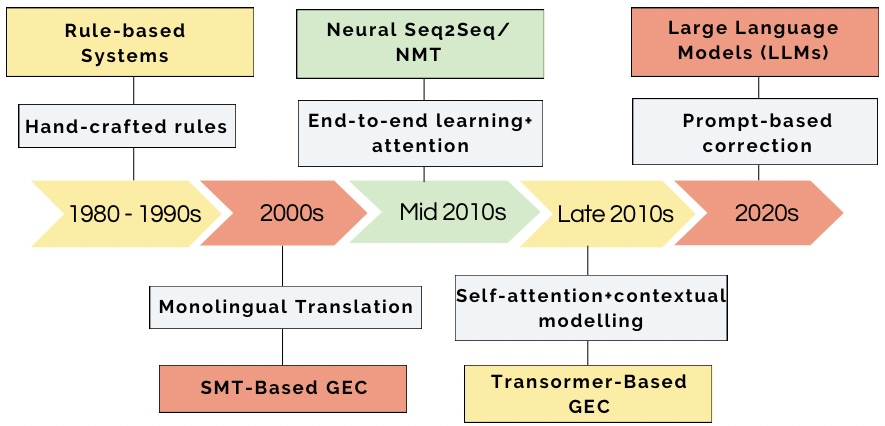
\includegraphics[width=\textwidth]{figures/evolution_of_gec.PNG}
    \caption{Evolution of Grammatical Error Correction Approaches}
    \label{fig:gec-timeline}
\end{figure}

\section{Evaluation in GEC: Metrics and Limitations}

As GEC systems moved from rule-based approaches to neural and Transformer architectures, evaluation frameworks developed alongside them. Reliable metrics are needed for benchmarking and model comparison. The difficulty is that correction quality is not always a single target, because one learner sentence may have several valid revisions. This section reviews the main evaluation metrics and explains why they are limited for unnecessary changes beyond minimal grammatical correction.

\subsection{ERRANT and the M\textsuperscript{2} Scorer}

One of the earliest and most widely adopted evaluation metrics in GEC is the M\textsuperscript{2} (MaxMatch) scorer, introduced by Dahlmeier and Ng \cite{dahlmeier-ng-2012-better}. The M\textsuperscript{2} scorer evaluates system outputs by aligning proposed edits with gold-standard human annotations and computing an F-score over matched edits. It became the official evaluation metric for the CoNLL-2014 shared task \cite{ng-etal-2014-conll} and remains a standard benchmark in subsequent research.

Unlike sentence-level comparison, M\textsuperscript{2} is edit-based: it extracts edits from system outputs and measures how many align with gold edits. Performance is typically reported using precision, recall, and the weighted $F_{0.5}$ score.

\paragraph{Precision.}
Precision measures the proportion of system edits that are correct:
\[
\text{Precision} = \frac{\text{Correct Edits}}{\text{System Edits}}
\]
High precision indicates that proposed corrections are usually valid.

\paragraph{Recall.}
Recall measures the proportion of gold edits successfully identified:
\[
\text{Recall} = \frac{\text{Correct Edits}}{\text{Gold Edits}}
\]
High recall indicates that the system captures a large share of existing errors.

\paragraph{$F_{0.5}$ Score.}
Because unnecessary corrections may reduce text quality, the GEC community commonly reports the $F_{0.5}$ score, which weights precision more heavily than recall:
\[
F_{0.5} =
\frac{(1 + 0.5^2)\cdot \text{Precision} \cdot \text{Recall}}
{0.5^2 \cdot \text{Precision} + \text{Recall}}
\]
The use of $F_{0.5}$ reflects a practical preference for avoiding false positives (unnecessary edits), as excessive corrections may degrade text quality \cite{ng-etal-2014-conll}.

Despite its standardisation benefits, M\textsuperscript{2} relies on a limited set of gold references. Valid alternative corrections may be penalised if they do not precisely match annotated edits. This limitation becomes more visible in neural systems, where outputs can be fluent but structurally different from the reference \cite{napoles-etal-2017-jfleg}.

To improve diagnostic capability, Bryant et al.\ introduced the ERRANT toolkit \cite{bryant-etal-2017-automatic}. ERRANT performs automatic alignment between the original learner sentence and its corrected counterpart using a linguistically informed algorithm. It extracts the minimal edits required to transform the source into the correction and assigns each edit to a standardised taxonomy of fine-grained error types (e.g., missing, replacement, unnecessary, and word-order errors). This structured representation enables per-error-type performance analysis and supports interpretable, edit-based evaluation beyond aggregate scoring. However, because ERRANT remains fundamentally alignment-based, it retains the same dependency on gold annotations and the same primary focus on grammatical accuracy, without explicitly accounting for over-correction risk.

\subsection{Limitations of Accuracy-Only Evaluation}

Edit-based metrics such as M\textsuperscript{2} and ERRANT assume that closer alignment with annotated edits corresponds to improved system quality. However, multiple valid corrections may exist, particularly when lexical or structural variation is possible. The JFLEG corpus \cite{napoles-etal-2017-jfleg} demonstrates that fluency-oriented revisions often involve broader rephrasing rather than minimal edits.

Crucially, these metrics evaluate correctness but not proportionality. Systems may introduce changes beyond what is required for grammatical repair without substantial score penalties. As neural systems and LLMs become increasingly generative, this tendency towards broader rewriting becomes more pronounced \cite{loem2023exploringeffectivenessgpt3grammatical}.

In educational contexts, this mismatch matters. Excessive rewriting can obscure learner constructions and reduce opportunities for noticing and reflection, processes central to second language acquisition theory \cite{schmidt1990role}. Optimising for precision, recall, and $F_{0.5}$ therefore does not necessarily mean that the output is pedagogically useful. This is why the present project uses complementary measures that look at the extent of textual modification as well as grammatical accuracy.

\subsection{Measuring Textual Change and Minimality}

To complement accuracy-based evaluation, other metrics can estimate how much a corrected sentence deviates from the original input.

\subsubsection{Edit Distance and Minimality}

Levenshtein distance \cite{levenshtein1966binary} measures the minimum number of insertions, deletions, and substitutions required to transform one string into another. In GEC, word-level edit distance provides a direct measure of correction magnitude: fewer edits suggest minimal intervention, while many edits indicate broader rewriting.

However, edit distance measures surface change only. It does not determine whether changes were necessary for grammatical correctness or whether they reflect unnecessary modification.

\subsubsection{BLEU and Its Limitations}

BLEU \cite{papineni2002bleu} evaluates n-gram overlap between a system output and one or more reference corrections. Although it is widely used in machine translation, BLEU has limitations for GEC. Because multiple valid corrections may exist, lexical differences can reduce overlap even when the correction is appropriate. BLEU also does not explicitly account for minimality: a heavily rewritten but fluent sentence may still achieve substantial n-gram overlap.

\subsubsection{SARI and Retention-Sensitive Metrics}

SARI \cite{xu2016optimizing}, originally developed for text simplification, evaluates additions, deletions, and retained (``kept'') words. Importantly, SARI explicitly rewards systems that preserve appropriate parts of the original learner sentence. This makes it conceptually relevant for minimal-edit GEC, as it provides a signal of how much original content is retained.

\subsubsection{Structural and Lexical Change Indicators}

Beyond edit counts and n-gram overlap, additional measures can capture broader changes in sentence structure and vocabulary. Lexical diversity metrics, such as Type--Token Ratio (TTR), measure vocabulary variation, while readability indices such as the Flesch--Kincaid Grade Level \cite{kincaid1975derivation} estimate structural complexity. Syntactic features, including sentence length and part-of-speech distribution, further reflect structural modification. Cosine similarity over lexical and syntactic feature vectors provides a quantitative estimate of similarity between the original and corrected sentences \cite{koppel2009computational}. Fluency-oriented indicators are also relevant because not every surface change is equally undesirable: a correction that preserves meaning and improves fluency may have greater pedagogical utility than a rewrite that changes wording without clear benefit.

These measures do not directly evaluate correctness. Instead, they provide indirect signals of how much the corrected sentence departs from the original and whether that departure appears useful. For this dissertation, that makes them useful for estimating potential over-correction risk, rather than for judging stylistic quality in isolation.

\subsubsection{Worked Example}

Consider:
\begin{figure}[h]
    \centering
    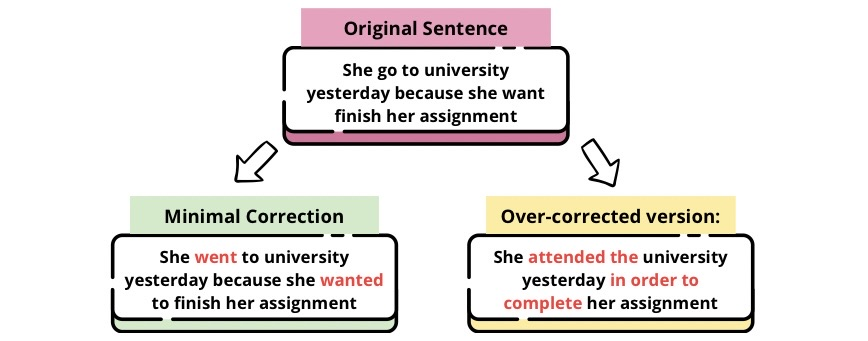
\includegraphics[width=\textwidth]{figures/minimal_vs_overcorrection.PNG}
    \caption{Minimal vs Over-Corrected Sentence}
    \label{fig:gec-example}
\end{figure}

The minimal correction introduces only necessary grammatical changes. Word-level edit distance remains low, and structural similarity to the original learner sentence is largely preserved.

In contrast, the over-corrected version replaces multiple lexical items (``went'' to ``attended'', ``because'' to ``in order to'', ``finish'' to ``complete'') and alters phrasing. Edit distance increases, readability and lexical properties shift, and similarity to the original decreases.

BLEU may still assign reasonable scores to both outputs due to lexical overlap, whereas SARI would more strongly reward retention in the minimal version. This example illustrates that grammatical correctness alone does not distinguish minimal correction from unnecessary rewriting.

\subsubsection{Comparative Summary of Metrics}

\begin{table}[h]
\centering
\caption{Comparison of Evaluation Metrics for GEC and Textual Change}
\label{tab:metric_comparison}
\begin{tabular}{|p{3cm}|p{4cm}|p{4cm}|}
\hline
\textbf{Metric} & \textbf{Measures} & \textbf{Limitation in GEC Context} \\
\hline
M\textsuperscript{2} / ERRANT & Edit alignment accuracy & Does not penalise unnecessary rewriting \\
\hline
Levenshtein Distance & Magnitude of surface change & Cannot distinguish necessary vs unnecessary edits \\
\hline
BLEU & N-gram overlap & Penalises valid alternatives; insensitive to minimality \\
\hline
SARI & Add/Delete/Keep operations & Designed for simplification, not grammar \\
\hline
TTR & Lexical diversity change & Sensitive to text length \\
\hline
Flesch--Kincaid & Readability change & Indirect proxy for structural modification \\
\hline
Similarity Metrics & Structural/lexical overlap & Requires feature engineering \\
\hline
\end{tabular}
\end{table}

Traditional edit-based metrics remain useful for benchmarking grammatical accuracy, but they are not sufficient for evaluating over-correction risk. This is why the later experiments combine ERRANT with change-based and utility-sensitive measures.

\section{Large Language Models in GEC}

The move from task-specific neural architectures to large-scale pre-trained language models changes how GEC can be approached. Earlier systems were trained directly on parallel corpora of erroneous and corrected sentences, learning to map learner input to gold-standard revisions. Large language models (LLMs), by contrast, acquire broad linguistic competence through large-scale self-supervised pre-training, typically by predicting missing or subsequent words across massive text corpora without manual annotation.

This makes zero-shot and few-shot correction possible without task-specific fine-tuning. Instead of retraining model parameters for GEC, correction behaviour can be elicited through natural language instructions alone.

\subsection{From Fine-Tuned Models to Prompt-Based GEC}

Traditional neural GEC systems relied on supervised fine-tuning using annotated learner corpora such as NUCLE and W\&I + LOCNESS \cite{ng-etal-2014-conll,bryant-etal-2019-bea}. These systems were optimised explicitly for edit-based metrics such as $F_{0.5}$, and their performance was constrained by the size and diversity of available annotated datasets.

Large Transformer-based models, including GPT-3 \cite{NEURIPS2020_1457c0d6}, showed that autoregressive language models can perform new tasks through in-context learning. In this setting, the model adapts to a task based on instructions and optional examples in the prompt, without updating its internal parameters.

In GEC, this enables prompt-based correction. Zero-shot prompting provides only task instructions (e.g., ``Correct grammatical errors''), while few-shot prompting includes example input--output pairs that illustrate the desired behaviour \cite{NEURIPS2020_1457c0d6}. Empirical studies show that LLMs can achieve competitive correction performance under these conditions despite the absence of task-specific training \cite{loem2023exploringeffectivenessgpt3grammatical}. This reduces dependence on annotated corpora and simplifies deployment across domains.

However, prompt-based GEC differs from supervised encoder--decoder systems. Because LLMs are trained to generate fluent and plausible continuations rather than to minimise edits, their outputs are influenced by instruction phrasing and contextual framing. Prompt design therefore becomes one of the main ways to influence correction granularity and the extent of unnecessary rewriting.

\subsection{Advantages of LLM-Based GEC}

LLM-based GEC is attractive for three reasons: fluency, generalisation, and adaptability.

\subsubsection{Fluency and Contextual Coherence}

Pre-trained on extensive and diverse corpora using next-token prediction objectives \cite{NEURIPS2020_1457c0d6}, LLMs develop strong syntactic and discourse modelling capabilities. As a result, their corrections are typically well-formed and contextually coherent.

Empirical studies report that GPT-style models not only resolve surface-level grammatical errors but also improve overall naturalness and readability \cite{loem2023exploringeffectivenessgpt3grammatical}. Compared to earlier SMT or fine-tuned neural systems, LLM outputs often exhibit more globally consistent phrasing.

\subsubsection{Generalisation Beyond Annotated Corpora}

Unlike fine-tuned systems limited to annotated learner datasets \cite{ng-etal-2014-conll,bryant-etal-2019-bea}, LLMs leverage knowledge acquired from large-scale heterogeneous pre-training data \cite{NEURIPS2020_1457c0d6}. Through prompting alone, they can perform GEC without direct exposure to task-specific corpora.

This broader linguistic coverage may help with error types that are underrepresented in benchmark datasets. The limitation is that pedagogical alignment remains uncertain, especially when fluency improvements extend beyond minimal grammatical correction and introduce unnecessary modifications.

\subsubsection{Adaptability Through Prompt Engineering}

Prompt-based systems are dynamically controllable through instruction design. Modifying phrasing, role specification, or illustrative examples can influence correction scope \cite{liu2023pretrain}. For instance, instructions such as ``Correct only grammatical errors without changing wording unnecessarily'' may encourage more constrained outputs.

This flexibility allows rapid adaptation without retraining and reduces computational cost. However, such adaptability also introduces behavioural variability, as small changes in prompt wording may lead to substantially different corrections, including variation in over-correction risk.

\subsection{Known Weaknesses of LLM-Based GEC}

Despite these strengths, LLM-based GEC exhibits limitations rooted in its generative training objective. Three recurring concerns are hallucination, over-editing, and prompt instability.

\subsubsection{Hallucination}

Hallucination refers to the introduction of content that is not present or implied in the input sentence \cite{maynez2020faithfulness}. In GEC, this may manifest as semantic additions, altered meaning, or inserted clarifications. Because LLMs prioritise plausibility and fluency over strict edit alignment \cite{NEURIPS2020_1457c0d6}, even subtle semantic shifts can compromise faithfulness to learner intent.

\subsubsection{Over-Editing and Loss of Minimality}

LLMs may over-edit by rephrasing clauses or substituting vocabulary to enhance fluency \cite{loem2023exploringeffectivenessgpt3grammatical}. While this can improve perceived readability, it may reduce minimality and transparency in educational contexts by introducing unnecessary changes beyond grammatical correction. A detailed discussion of fluency bias and over-correction is provided in Section~\ref{sec:fluency-bias}.

\subsubsection{Instability Across Prompts}

Because correction behaviour is governed by natural language instructions rather than explicit task-specific training, outputs are sensitive to prompt formulation \cite{liu2023pretrain}. Small variations in wording or example selection can alter both correction accuracy and the degree of rewriting.

Carefully engineered prompts may encourage minimal edits, but they do not guarantee consistent behaviour. This is the reason the present study compares prompt-induced variation in rewriting behaviour rather than assuming that a constraint in the prompt will always be followed.

\subsection*{Summary}

LLMs offer substantial improvements in fluency, generalisation, and adaptability compared to earlier GEC systems. However, their generative nature introduces trade-offs between naturalness and faithfulness. Hallucination and prompt sensitivity highlight the need to evaluate not only grammatical accuracy but also over-correction risk, particularly in educational contexts where minimal and transparent correction is essential.

\section{Fluency Bias, Over-Correction, and Educational Alignment}
\label{sec:fluency-bias}

The increasing use of LLMs in GEC has drawn attention to a tendency often described as \textit{fluency bias}. Whereas earlier GEC systems were optimised for edit-based correction, generative LLMs are trained to produce probable and natural-sounding text. This creates a tension between grammatical correction and changes that go beyond minimal repair, particularly in educational contexts.

\subsection{Defining Fluency Bias}

Fluency bias refers to the tendency of LLMs to prioritise naturalness and coherence, even when such modifications extend beyond necessary grammatical correction. During pre-training, models learn to predict the next (or masked) word across large corpora of fluent text \cite{NEURIPS2020_1457c0d6,NIPS2017_3f5ee243}. This objective rewards globally plausible sequences rather than minimal, localised edits.

In GEC, fluency bias manifests as clause restructuring, lexical substitution, or syntactic reformulation beyond morpho-syntactic correction. Although such revisions often enhance readability, they may introduce unnecessary changes that alter the learner's original phrasing. This diverges from the minimal-edit paradigm underlying shared tasks such as CoNLL-2014 \cite{ng-etal-2014-conll}, where corrections are assumed to be proportional to the error.

Empirical studies document systematic rewriting in GPT-based systems \cite{loem2023exploringeffectivenessgpt3grammatical}, while fluency-oriented datasets such as JFLEG similarly prioritise naturalness over minimality \cite{napoles-etal-2017-jfleg}. From an optimisation perspective, fluency bias reflects a mismatch between models trained for fluent sequence generation and pedagogical settings that value transparent, minimal intervention.

\subsection{Over-Correction as Structural Consequence}

Over-correction is the observable manifestation of fluency bias. Systems introduce lexical or structural changes beyond resolving grammatical errors, producing outputs that are grammatically valid yet unnecessarily different from the original phrasing.

Over-correction is not inherently incorrect, and it is difficult to define or measure directly because some broad revisions may be useful in context. Evaluation metrics such as M\textsuperscript{2} and ERRANT reward grammatical accuracy without explicitly penalising unnecessary rewriting. As a result, systems with strong fluency bias may achieve competitive $F_{0.5}$ scores while still moving away from minimal-edit principles.

Comparative analyses suggest that fine-tuned encoder--decoder models trained on annotated learner corpora tend to produce more localised edits aligned with gold references \cite{ng-etal-2014-conll,bryant-etal-2019-bea}, whereas LLM outputs display greater lexical and structural variation despite similar quantitative performance. Equivalent scores may therefore mask qualitatively different correction behaviours.

\subsection{Pedagogical and Alignment Implications}

In second-language (L2) contexts, over-correction carries significant pedagogical implications. While fluency-enhancing revisions may improve surface quality, they can conflict with core learning principles.

Extensive reformulation may obscure the learner's original wording and reduce transparency of feedback. In contrast, minimal correction encourages direct comparison between incorrect and corrected forms, which is essential to language acquisition theory \cite{schmidt1990role}. Fluency-biased rewriting introduces multiple simultaneous changes, potentially obscuring the locus of error.

Repeated exposure to fully rewritten sentences may also foster dependency, reducing learner engagement in active revision \cite{ke2019automated}. Educational feedback should scaffold learning rather than replace cognitive effort.

These concerns reflect a broader alignment challenge. In educational GEC, the intended objective is targeted grammatical repair with minimal necessary modification. For LLMs, the learned objective is fluent sequence generation. Fluency bias therefore creates a mismatch between model optimisation and instructional goals.

\subsection{Illustrative Example}

\begin{figure}[h]
    \centering
    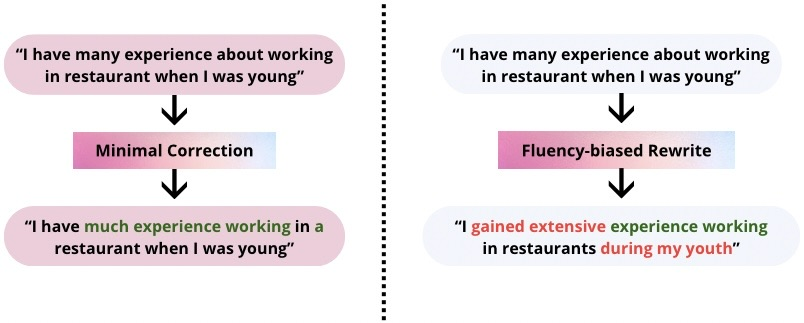
\includegraphics[width=\textwidth]{figures/minimal_vs_fluency.PNG}
    \caption{Minimal Correction vs Fluency-biased Rewrite}
    \label{fig:gec-timeline}
\end{figure}

The minimal correction adjusts only necessary grammatical elements while preserving structural similarity, facilitating transparent comparison. The fluency-biased rewrite introduces lexical substitution and structural reformulation, increasing the degree of modification and reducing visibility of the original error.

\vspace{4.0cm}

\subsubsection{Comparative Summary}

\begin{table}[htbp]
\centering
\caption{Pedagogical Comparison: Minimal Correction vs Fluency-Biased Rewrite}
\label{tab:pedagogical_comparison}
\begin{tabular}{|p{4cm}|p{4cm}|p{4cm}|}
\hline
\textbf{Dimension} & \textbf{Minimal Correction} & \textbf{Fluency-Biased Rewrite} \\
\hline
Edit Scope & Localised changes & Structural reformulation \\
\hline
Learner Wording & Preserved & Modified \\
\hline
Error Transparency & High & Reduced \\
\hline
Support for Noticing & Facilitates comparison & May obscure error locus \\
\hline
Dependency Risk & Lower & Higher \\
\hline
\end{tabular}
\end{table}

\section{Prompt Engineering as Behavioural Control}

In the absence of task-specific fine-tuning, prompt engineering becomes the primary mechanism for influencing how LLMs perform GEC. Prompt design therefore functions as behavioural control: it shapes how the model interprets task scope and how strongly it prioritises minimal correction over broader rewriting.

Prompt engineering refers to the strategic formulation of instructions and contextual examples to influence model outputs without modifying internal parameters \cite{liu2023pretrain}. Unlike supervised fine-tuning, which adjusts model weights through gradient optimisation, prompting operates entirely through input conditioning \cite{NEURIPS2020_1457c0d6}. In GEC, prompt formulation may determine whether the model performs minimal grammatical repair or introduces unnecessary modifications beyond what is required.

\subsection{Prompting Strategies for Behavioural Control}

Prompt-based control of LLM behaviour can be grouped into instruction-based, constraint-based, role-based, and example-driven prompting. These approaches overlap in practice, but they differ in how much guidance and structure they give to the model.

\subsubsection{Instruction-Based Prompts}

Instruction-based prompting uses natural-language directions to define the scope of the task. In zero-shot configurations, the model receives only an instruction and the input sentence, without demonstration examples \cite{NEURIPS2020_1457c0d6}. The clarity and specificity of the instruction therefore play a central role in shaping model behaviour.

For GEC, a generic instruction such as:

\begin{quote}
``Correct the following sentence.''
\end{quote}

leaves the scope of correction underspecified. The model may interpret ``correct'' as encompassing grammar, fluency, vocabulary refinement, and broader rewriting, potentially triggering unnecessary modifications.

By contrast, a more explicit formulation such as:

\begin{quote}
``Correct only grammatical errors. Do not change word choice or sentence structure unless strictly necessary.''
\end{quote}

attempts to align the model's behaviour with minimal-edit principles. Research on instruction tuning demonstrates that LLMs are sensitive to task framing and that explicit constraints embedded within instructions can influence output characteristics \cite{wei2022finetuned,liu2023pretrain}. However, the reliability of such constraints in reducing over-correction within GEC remains insufficiently examined.

\subsubsection{Constraint-Based Prompts}

Constraint-based prompting extends instruction-based approaches by introducing operational limits on permissible edits. Rather than simply defining the task, these prompts specify how correction should occur. For instance, constraints may restrict edits to particular error types (e.g., verb tense or article usage), prohibit synonym substitution, or require preservation of syntactic structure unless grammatically necessary.

This approach aligns with the minimal-edit paradigm historically emphasised in shared tasks such as CoNLL-2014 \cite{ng-etal-2014-conll}. By narrowing the permissible transformation space, constraint-based prompts aim to reduce unnecessary rewriting and lexical substitution.

Constraints still function as soft guidance rather than enforceable rules. Because LLMs remain optimised for generative coherence, adherence to constraints is probabilistic rather than deterministic \cite{liu2023pretrain}. Overly restrictive prompts may also suppress legitimate structural corrections, particularly in sentences where grammatical and phrasing issues are intertwined. Evaluating constraint-based prompts therefore requires balancing minimal modification against correction completeness.

\subsubsection{Role-Based Prompts}

Role-based prompting introduces behavioural framing by assigning the model a specific identity or perspective. Instead of merely issuing instructions, the prompt situates the model within a defined role, for example:

\begin{quote}
``You are an English teacher providing minimal grammatical corrections to an L2 learner.''
\end{quote}

Role conditioning has been shown to influence tone, lexical choices, and interpretive stance in LLMs \cite{wei2022finetuned,liu2023pretrain}. Framing the model as an educator rather than an editor may implicitly encourage more restrained corrections and better alignment with pedagogical goals.

Role effects emerge from latent associations acquired during pre-training, so they may be less predictable than explicit constraints. Role-based prompts may influence output style and explanatory framing, but tendencies towards broader rewriting can still persist \cite{NEURIPS2020_1457c0d6}. Role framing alone is therefore unlikely to eliminate fluency bias, although it may complement other control mechanisms.

\subsubsection{Few-Shot and Example-Driven Prompts}

Few-shot prompting adds demonstration examples to the prompt \cite{NEURIPS2020_1457c0d6}. Rather than relying only on abstract instructions, the model is shown explicit input--output pairs that illustrate the desired form of correction. These examples act as templates, guiding the model towards similar transformations.

In the context of GEC, example-driven prompts can demonstrate minimal-edit behaviour directly. Research on in-context learning indicates that few-shot examples can shape model outputs, sometimes more strongly than high-level instructions alone \cite{liu2023pretrain}. Factors such as example ordering, similarity to the input, and diversity have been shown to affect performance \cite{wei2022finetuned}.

However, few-shot prompting introduces methodological challenges. Longer prompts increase computational cost and approach context-length constraints. Additionally, poorly selected examples may encourage consistent rewriting patterns that go beyond minimal correction. Careful control of example content is therefore necessary to ensure that behavioural effects result from prompt structure rather than implicit data leakage.

\subsubsection*{Synthesis and Research Focus}

These prompting strategies control different parts of the correction request. Instructions define the task, constraints narrow the allowed edits, role framing changes the stance of the response, and examples show the model what kind of correction is expected. Prior work suggests that prompting can influence correction behaviour, but it is still unclear how far it can reduce unnecessary rewriting in learner-facing GEC.

The present project does not attempt to resolve prompt controllability in general. It asks a narrower question: whether a small set of structured prompting strategies can reduce over-correction risk, relative to a simple baseline prompt, while maintaining broadly comparable grammatical correction performance in an L2-focused setting. This limited focus matches the controlled empirical study reported in later chapters.

\subsection{Prompt Sensitivity and Behavioural Stability}

Prompt fragility describes the phenomenon whereby outputs remain highly sensitive to prompt formulation, even when prompting is intended to provide behavioural control \cite{liu2023pretrain}.

\subsubsection{Prompt Fragility}

Because in-context learning modifies behaviour through conditioning rather than parameter updates \cite{NEURIPS2020_1457c0d6}, minor variations in wording or structure can activate different latent response patterns. In GEC, replacing ``correct grammatical errors'' with ``improve the sentence'' may shift output from minimal repair towards broader rewriting.

\subsubsection{Controllability}

Controllability refers to the consistency with which prompts enforce constraints. Empirical evidence suggests that constraint adherence is probabilistic \cite{wei2022finetuned,liu2023pretrain}. Prompts therefore operate as soft steering mechanisms rather than strict rule systems.

\subsubsection{Alignment Challenges}

Prompt sensitivity reflects a broader alignment issue: the intended objective (minimal grammatical repair) may diverge from the model's learned objective (fluent sequence generation) \cite{NEURIPS2020_1457c0d6}. This structural misalignment contributes directly to fluency bias and unnecessary rewriting. Understanding the limits of prompt controllability is therefore essential for determining whether behavioural regulation through prompting is sufficient for educational deployment.

\subsubsection*{Conceptual Control Framework}

In zero-shot and few-shot settings, behavioural control exists primarily at the prompt specification stage. The input sentence remains fixed and model parameters unchanged. Prompt engineering therefore constitutes the principal adjustable interface for influencing correction behaviour.

Figure~\ref{fig:prompt_pipeline} illustrates this control locus.

\begin{figure}[htbp]
\centering
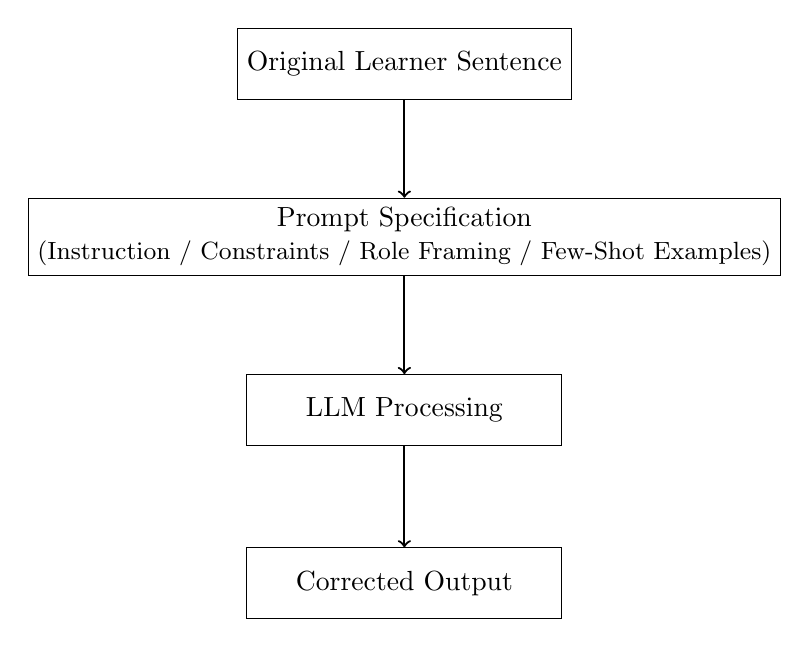
\begin{tikzpicture}[
  node distance=2.2cm,
  every node/.style={draw, rectangle, align=center, minimum width=4cm, minimum height=0.9cm}
]
\node (input) {Original Learner Sentence};
\node (prompt) [below of=input] {Prompt Specification \\ \small (Instruction / Constraints / Role Framing / Few-Shot Examples)};
\node (model) [below of=prompt] {LLM Processing};
\node (output) [below of=model] {Corrected Output};

\draw[->, thick] (input) -- (prompt);
\draw[->, thick] (prompt) -- (model);
\draw[->, thick] (model) -- (output);
\end{tikzpicture}
\caption{Conceptual Control Points in Prompt-Based Grammatical Error Correction}
\label{fig:prompt_pipeline}
\end{figure}

This literature motivates the experimental design of the present study: the later chapters test whether structured prompting changes the balance between grammatical accuracy and over-correction risk.

\section{Ethical and Professional Considerations}

Deploying LLM-based GEC in educational contexts raises ethical and professional issues beyond technical performance. Although this dissertation focuses on regulating over-correction through prompt engineering, a real system would also need to consider learner agency, transparency, fairness, and data handling.

\subsection{Human--AI Interaction, Transparency, and Learner Agency}

LLM-based writing systems can generate fully revised text rather than highlighting isolated rule violations. This shifts the locus of agency in the revision process: instead of guiding learners towards self-correction, the system may effectively perform revision on their behalf.

Human--AI interaction research emphasises that AI systems should augment, rather than replace, human cognitive effort \cite{amershi2019guidelines}. In educational contexts, feedback is most useful when it supports learning rather than simply automating revision. Studies of automated writing evaluation show that learner uptake depends on clarity, perceived fairness, and opportunities for iterative revision \cite{ke2019automated}. Overly broad or opaque corrections may therefore reduce reflective engagement, particularly when they involve unnecessary rewriting beyond grammatical repair.

Transparency refers to the extent to which users can understand what a system has changed and why. Earlier rule-based systems provided relatively interpretable transformations linked to identifiable grammatical rules, whereas LLMs operate through high-dimensional statistical representations that lack inherent interpretability \cite{NIPS2017_3f5ee243}. Prompting can influence correction scope, but it does not inherently provide explanations. Without highlighted edits or rationales, learners may struggle to infer the underlying grammatical principles. Responsible AI frameworks emphasise transparency, accountability, and user awareness in high-impact domains such as education \cite{floridi2018ai4people}.

\subsection{Risk Analysis}

Integrating LLM-based correction tools into L2 learning environments introduces identifiable risks that warrant mitigation.

\subsubsection{Learner Dependency and Reduced Critical Engagement}

When systems provide fully rewritten sentences rather than targeted corrections, learners may rely on automated revision instead of engaging in active error analysis. Research on automated writing evaluation raises similar concerns: excessive automation can reduce reflective learning and learner autonomy \cite{ke2019automated}. Accepting corrections without examining underlying rules may also weaken metalinguistic awareness. Schmidt's noticing hypothesis emphasises that conscious attention to linguistic form supports acquisition \cite{schmidt1990role}. Extensive or unnecessary rewriting may therefore limit learning by obscuring the specific source of error.

\subsubsection{Linguistic Homogenisation and Bias}

LLMs are trained on large-scale text corpora that reflect dominant linguistic norms. As a result, correction outputs may implicitly standardise writing towards particular registers or dialects \cite{NEURIPS2020_1457c0d6}. In multicultural educational settings, unnecessary rewriting may marginalise legitimate variation and reduce diversity of expression. Ensuring fairness therefore requires distinguishing genuine grammatical violations from acceptable linguistic variation \cite{floridi2018ai4people}.

\subsubsection{Data Privacy and Security}

Processing learner writing introduces privacy considerations, particularly when texts contain personal or sensitive information. This project uses an existing anonymised corpus rather than collecting new participant data. The practical risk is therefore lower than in a deployed classroom system, but secure storage, limited retention, and careful handling of model inputs remain necessary safeguards.

\subsubsection{Academic Integrity and Misuse}

Although minimal grammatical correction differs from content generation, the boundary between editing and rewriting can become blurred. Without clear usage guidelines, AI-assisted tools may be used in ways that compromise authorship transparency or academic integrity, particularly in assessment contexts.

\subsubsection*{Structured Risk Assessment}

Table~\ref{tab:risk_assessment} summarises the principal risks and corresponding mitigation strategies.

\begin{table}[htbp]
\centering
\caption{Risk Assessment for LLM-Based Grammatical Error Correction}
\label{tab:risk_assessment}
\begin{tabular}{|p{4cm}|p{3cm}|p{3cm}|p{4cm}|}
\hline
\textbf{Risk} & \textbf{Likelihood} & \textbf{Impact} & \textbf{Mitigation Strategy} \\
\hline
Learner Dependency & Medium & High & Emphasise minimal correction; encourage revision comparison \\
\hline
Reduced Critical Engagement & Medium & High & Provide highlighted edits; integrate explanatory feedback \\
\hline
Linguistic Homogenisation & Medium & Medium & Limit unnecessary rewriting and preserve learner wording where possible \\
\hline
Data Privacy Breach & Low--Medium & High & Anonymise data; limit storage; ensure regulatory compliance \\
\hline
Academic Misuse & Medium & High & Establish clear usage guidelines; distinguish correction from generation \\
\hline
\end{tabular}
\end{table}

\subsection{Study Safeguards}

In this study, the learner data are handled in anonymised form, and no additional personal information is collected. The experiments store only the source sentences, prompt labels, model outputs, and evaluation results needed for the analysis. Because the model calls use an external API, the study avoids adding any participant identifiers beyond the existing anonymised corpus records.

\vspace{3cm}

\section{Identified Research Gaps}

Despite recent progress in GEC and LLM-based approaches, several gaps remain at the intersection of evaluation, controllability, and pedagogy. These gaps matter for this project because grammatical accuracy alone is not enough in learner-facing correction; preservation of learner wording is also part of the feedback problem.

\subsection{Gap 1: Limited Evaluation of Unnecessary Changes}

Most GEC evaluation frameworks prioritise grammatical accuracy. Metrics such as M\textsuperscript{2} and ERRANT measure how closely system edits align with annotated references \cite{dahlmeier-ng-2012-better,bryant-etal-2017-automatic}, but they do not directly assess whether additional lexical or structural changes were necessary. As a result, systems may achieve competitive scores even when they introduce broader rewriting than the task pedagogically requires.

Although fluency-oriented resources such as JFLEG \cite{napoles-etal-2017-jfleg} acknowledge that valid correction may extend beyond minimal edits, they also reinforce evaluation practices in which naturalness can overshadow proportionality. Relatively few studies combine standard GEC metrics with complementary measures of textual change, such as edit distance, lexical diversity, readability, or similarity-based measures. This limits the ability to evaluate whether a system preserves learner wording while performing grammatical correction.

\subsection{Gap 2: Limited Empirical Characterisation of Over-Correction}

Fluency bias and over-correction have been identified conceptually in prior work \cite{loem2023exploringeffectivenessgpt3grammatical}, but detailed empirical characterisation remains limited. Existing studies often focus on overall correction performance, with less attention to how unnecessary rewriting manifests at the sentence level or how it varies across prompting conditions.

More specifically, the literature provides limited evidence on whether structured prompts can reduce the overall degree of rewriting relative to a simple baseline prompt, and on how this reduction can be observed through measures of textual change. While some studies discuss controllability in broad terms, fewer provide controlled comparisons of prompt designs specifically in relation to minimality and unnecessary modification in learner writing.

\subsection{Gap 3: Limited Study of Prompt-Based Control in Pedagogically Framed GEC}

Prompt engineering has been widely studied in general NLP \cite{liu2023pretrain,wei2022finetuned}, but its application to learner-oriented GEC remains underexplored. Much of the LLM-based GEC literature focuses on feasibility, benchmark performance, or general prompt effectiveness rather than on whether prompt design can support pedagogically appropriate behaviour, such as preserving learner wording and avoiding unnecessary reformulation.

In particular, there are still relatively few controlled studies that bring together prompt design, evaluation of textual modification, and educational considerations. Prompt effectiveness in general text generation does not automatically mean that the output is appropriate for L2 feedback.

\subsection*{Synthesis and Positioning of the Present Study}

These gaps lead to the narrower problem addressed in this dissertation: current GEC evaluation practice does not adequately account for over-correction risk, and prompt-based work has not yet shown clearly how far structured prompts can moderate rewriting in learner-oriented settings.

The project addresses the problem in three bounded ways. First, it supplements conventional ERRANT-based accuracy evaluation with measures that track divergence from the source sentence. Second, it compares a small set of prompting strategies under controlled conditions to test whether prompt formulation affects the degree of rewriting. Third, it interprets these findings in relation to pedagogical concerns about transparency, minimality, and preservation of learner wording.

The contribution of this dissertation is therefore not a complete theory of over-correction, nor a full pedagogical evaluation of LLM-based GEC. Its contribution is more specific: it provides a controlled empirical case study showing how prompt design can influence the balance between grammatical correction and over-correction risk, and it uses an evaluation perspective that is more sensitive to potential over-correction than accuracy-only reporting.

The literature therefore leaves a practical question for this project: can a small set of structured prompts reduce indicators of over-correction risk relative to a simple baseline prompt? The dissertation answers this question through a controlled comparison using ERRANT-based accuracy metrics and change-sensitive measures based on the source sentence.
